\documentclass{article}

\usepackage[a4paper,margin=1in]{geometry}

\usepackage{mystyle}
\usepackage[sort,comma,numbers]{natbib}
\usepackage{algorithm}
\usepackage[noend]{algpseudocode}
\usepackage{hyperref}

\usepackage{subcaption}

\title{Storylines}

\begin{document}
\maketitle

\section{Introduction}
Modern generative models of text are extremely flexible, with huge amounts of parameters
trained on vast amounts of data \citep{brown2020language}.
However, these black-box text generation models may not be satisfactory in all text-generation
scenarios, especially when interpretability or control is necessary.
In such scenarios, a model with explicit structure would be more suitable,
as the structure would afford both interpretability and controllability.

Our goal is to design structured generative story models by modeling storylines.
Prior work has noted that including structure in the generative model improves coherence
\citep{yao2018storyline,fan2019structure}.
However, prior investigations into narrative structure use hand-crafted representations,
such as entity coreference or keywords.
We explore a different definition of what constitutes a storyline:
We hypothesize that storylines are composed of groups of sentences, or segments, that function
similar to motifs in biological sequences.
Motifs in biological sequences are recurring patterns that are believed to have
biological signifiance \citep{biomotif}.
For example, they may determine how protein interactions take place.
Analogously, we posit that storyline segments determine how a reader interprets
a story.

Modeling reader interpretation is very difficult, as eliciting such an interpretation from a human
would be very expensive.
Thankfully, biological sequence alignment algorithms offer a solution to this problem.
Biological sequence alignment algorithms find motifs without directly modeling
downstream effects, and only use similarity between elements of the sequences themselves.

Typically, these similarity measures are derived from manually-specified rules specific
to biological applications.
Our hypothesis, that similar storylines segments have a similar effect on readers,
implies that the similarity measure for storylines should be semantic.
We therefore turn to large pre-trained sentence representations \citep{reimers2019sbert},
as they have been shown to perform very well on related tasks such as natural language 
inference and entailment.

We perform an exploratory analysis of storyline induction by utilizing 
biological sequence alignment algorithms as well as large pretrained sentence representations.
We show that alignment algorithms built upon measures of semantic similarity 
are able to extract common structure from stories.

\section{Related Work}
Automatic story generation is a difficult task.
The best-performing language models are extremely flexible, but not specialized
for generating coherent stories.
Additionally, highly flexible black-box models are difficult to control,
as they were not designed with intervention in mind.
Prior work addresses this problem by using incorporating hand-designed proxies
of storylines, such as keywords \citep{yao2018storyline}
or information from classical NLP pipelines \citep{fan2019structure}.
Although effective at improving the generative model,
approaches that require specifying storyling representations
are unlikely to scale to many use-cases.

Work in structured molecule generation also benefits from a 
hierarchical generation process.
The structured generative model in \citet{wengong2020moleculemotif}
utilize graph motifs were useful for improving a generative model of molecules.
Although the motifs in molecules are graph-based, and therefore both
easier to identify and structurally different than the sequence motifs we consider,
the improvements to the generative model are significant.

A recent application of biological sequence algorithms
by \citet{alayrac2015align} applies techniques from alignment
to the problem of aligning instructional videos to textual narrations.
Analogous to storyline induction from multiple stories,
they aim to jointly align multiple narratives to video
in order to discover actions sequences.
Interestingly, they found that classical approaches
to sequence alignment are outperformed by modern optimization techniques.
Storylines are much more complex than action sequences from instructional videos,
as the intentions behind stories vary greatly.

\section{Background: Pairwise Sequence Alignment}
The goal of pairwise sequence alignment is to find a minimum cost alignment
between sequences of sentences $\bx_1$ and $\bx_2\in\Sigma^*$, where
sentences are represented by a vector in $\R^n$.
We additionally add a gap symbol `-' to $\Sigma$, such that 
$\Sigma = \R^n \cup \set{-}$.
We refer to elements of $\Sigma$ as tokens.

In order to align two stories, pairwise alignment extends edit distance
with a distance measure $d: \Sigma\times\Sigma\to\R$ that operates on pairs of tokens,
one from each story.
The best alignment is given by the following:
\begin{equation}
\label{eqn:align}
\argmin_\pi \sum_{(i, j) \in \pi} d(x_{1i},x_{2j}),
\end{equation}
where $\pi$ is a joint path through $\bx_1$ and $\bx_2$.
Valid paths are obtained by only inserting gaps into the original story
while preserving order.
Equation~\ref{eqn:align} can be solved exactly via dynamic programming.
Let $\bx^\pi_1,\bx^\pi_2$ be the gap-augmented stories obtained by following path $\pi$,
which are both of length $L$.
We refer to 
%\begin{equation}
$M = \begin{pmatrix}\bx^\pi_1 \\ \bx^\pi_2 \end{pmatrix}$
%\end{equation}
as the alignment.

When choosing a distance measure $d$, a key component is how the measure deals with gaps.
There are two approaches: 1) gaps correspond to insertion or deletions and 2) gaps
correspond to expansions or compressions.
Classical algorithms from biology, such as Needleman-Wunsch, model insertions and deletions,
as random mutations result in completely new elements that do not have a good interpretation
as an expansion or compression.
Other algorithms such as Dynamic Time Warping (DTW) model expansions and compressions,
since warping may occur due to various reasons such as sampling at different frequencies.
With stories, an example of expansion would be to split a long sentence into
shorter sentences.
It is possible to model both of these phenomena in the distance measure.
We assume that adding a sentence to a story, even if it builds on prior sentences,
adds new information and is semantically different from preceding sentences,
and therefore only model insertion and deletion.

\section{Problem Setup: Multiple Sequence Alignment}
In order to extract storylines, we would like to find patterns that are robust across
multiple stories. 
Unfortunately, methods for solving pairwise alignment are not directly applicable, since they
only consider pairs of stories.
Instead, we turn to the problem of multiple sequence alignment,
which generalizes alignment from pairs of stories to sets of stories.

Given a set of $K$ sequences,
a multiple alignment is a matrix $M \in \Sigma^{K \times L}$, given by:
\begin{equation}
M = \begin{pmatrix}
    \bx_1^\pi \\
    \vdots \\
    \bx_K^\pi
\end{pmatrix},
\end{equation}
where each $\bx_i^\pi$ is obtained by inserting gaps into the corresponding $\bx_i$
to ensure that each $\bx_i^\pi$ is of length $L$, as in pairwise alignment.

There are two common measures of quality for a multiple alignment:
1) the sum of pairs (SP) score and 2) the consensus error or Steiner distance.
All methods use the distance measure $d: \Sigma\times\Sigma\to\R$ from pairwise alignment.
The SP score is given by
\begin{equation}
\mathrm{SP}(M) = \sum_{l=1}^L \sum_{i=1}^K \sum_{j=i+1}^K d(M_{il}, M_{jl}),
\end{equation}
obtained by summing the pairwise distances between elements of $M$ in the same column.
The consensus error given a consensus sequence $\bz\in\Sigma^L$ is defined as follows:
\begin{equation}
\mathrm{CE}(M, \bz) = \sum_{l=1}^L \sum_{i=1}^K d(M_{il}, z_{l}),
\end{equation}
the sum of the distances from each element in a column to $z_l$.
The mean sequence $\bz\in\Sigma^L$ that minimizes this error is known as the consensus sequence.
Finally, the Steiner distance is closely related to the consensus error,
and can be computed without explicitly constructing a multiple alignment.
Let $D: \Sigma^* \times \Sigma^* \to \R$
be the distance measure obtained under global pairwise alignment using the token distance $d$,
so that $D$ operates on pairs of sequences.
The Steiner distance is given by
\begin{equation}
\mathrm{SD}(\mcX, \bz) = \sum_{i=1}^K D(\bx_i, \bz).
\end{equation}
The optimal consensus error, $\min_\bz\mathrm{CE}(M,\bz)$,
is equivalent to the optimal Steiner distance, $\min_{\bz}\mathrm{SD}(\mcX, \bz)$
\citep{gusfield1997}.
Additionally, the optimal Steiner sequence, $\arg\min_{\bz}\mathrm{SD}(\mcX, \bz)$,
is equivalent to the optimal consensus sequence, $\arg\min_\bz\mathrm{CE}(M,\bz)$,
up to spaces.
(Double check this last part carefully, maybe cut out consensus error definition.)

We utilize algorithms that optimize both the SP score and the Steiner distance.

\section{Methods}
As optimizing both the SP score and Steiner distance are NP-hard,
we resort to heuristic optimization methods.
We use a combination of three approaches: a progressive alignment method
inspired by a classical algorithm from computation biology,
an iterative averaging method similar to a popular algorithm from time-series analysis,
and a greedy hill climbing algorithm that operates in the space of Steiner sequences.

\subsection{Progressive Alignment}
Inspired by the progressive alignment algorithm
of \citet{fengdoolittle}, we first take a naive approach to approximating
a multiple sequence alignment.
Progressive alignments aim to optimize the SP score.

Given a set of sequences $\mcX$ and an ordering $\sigma$,
we progressively align the next sequence in the ordering to the
already aligned sequences.
Once a set of sequences are aligned, their columns of the alignment are frozen;
elements of new sequences must align to a whole column
from the existing alignment or a gap.
This is referred to as the `once a gap, always a gap' property \citep{fengdoolittle}.

In order to align a sequence to an existing alignment, we lift the definition of
the token distance $d$ to compare an element to a column of an alignment 
such that $d^+: \Sigma^*\times\Sigma\to\R$, as follows:
\begin{equation}
\label{eqn:dplus}
d^+(\by, x) = \sum_{j=1}^{|\by|} d(y_j, x).
\end{equation}
We can then extend pairwise global alignment with $d^+$, allowing us to
align the columns of an alignment to a token.
The full algorithm is given in Algorithm~\ref{alg:progressive}.

\begin{algorithm}[h]
\begin{algorithmic}
\State{Given: A set of sequences $\mcX = \set{\bx_i}_i$,
ordering $\sigma$, and extended distance measure $d^+$}
\State{Initialize alignment $M$ to $\bx_{\sigma(1)}$}
\ForAll{sequences $\bx_{\sigma(i)}$ in order $\sigma$}
    \State{Update $M = \Call{PairwiseAlign}{M, \bx_{\sigma(i)}, d^+}$ }
\EndFor
\Return{$M$}
\end{algorithmic}
\caption{\label{alg:progressive}
Progressive Alignment
}
\end{algorithm}

\subsection{An Iterative Averaging Algorithm}
Next, we propose an iterative averaging (IA)
algorithm which directly optimizes the Steiner distance.
The IA algorithm is inspired by the
DTW Barycenter Averaging (DBA) algorithm \citep{petitjean2011dba},
which iteratively computes pairwise alignments between a mean sequence $\bz$
and a set of sequences $\mcX$ then uses those alignments to recompute the mean sequence. 
As the DBA algorithm was designed to model expansion and compression, 
we adapt it for insertion and deletion.

The IA algorithm proceeds in a fashion similar to DBA.
We first construct a multiple alignment from the
pairwise alignments, then for each column of the multiple alignment
compute the token that minimizes the distance to each element within that column.
As we model insertions and deletions,
there is ambiguity when mapping the pairwise alignments to a joint multiple alignment.
Namely, there are multiple ways of aligning tokens from $\mcX$ that are all aligned to gaps
in $\bz$.
We resolve this ambiguity heuristically by inserting gaps in
the $\bx_i^\pi$ obtained by pairwise alignment with $\bz$
so that all tokens aligned to elements in $\bz$ are aligned.
The algorithm is detailed in Algorithm~\ref{alg:ia}.

\begin{algorithm}[h]
\begin{algorithmic}
\State{Given: A set of sequences $\mcX = \set{\bx_i}_i$
and distance measure $d$}
\State{Given: Initial mean string $\bz$}

\Function{IterativeAverage}{$\bz, \mcX, d$}
\ForAll{iterations}
    \ForAll{sequences $\bx_i \in \mcX$}
        \State{Compute pairwise alignments $M^i = \Call{PairwiseAlign}{\bx_i, \bz, d} \in \Sigma^{2\times L_i}$}
    \EndFor
    \State{Compute multiple alignment $M = \Call{Stack}{M^1, \ldots, M^K}$}
    \State{Update $\bz = \Call{Average}{M, d}$}
\EndFor
\Return{$M$}
\EndFunction

\Function{Stack}{$M^1, \ldots, M^K$}
\While{Non-gap elements of $\bz$ are not aligned in all $M^i_2$}
\State{Record column indices of $M^i_2$ that have a non-gap element of $\bz$}
\State{Insert $(-,-)$ columns to the left of the columns with non-gap elements from $\bz$
    for each $M^i$}
\EndWhile
\Return{$\begin{pmatrix}M^{1}_1\\\hdots\\M^{K}_1\end{pmatrix}$}
\EndFunction

\Function{Average}{$M, d$}
\State{Initialize $\bz\in\Sigma^{L}$}
\ForAll{columns $l$ in $M$}
\State{Set proposal $z'$ to the average non-gap representation of column $l$}
\State{Compute costs $c(z') = \sum_i d(M_{il}, z')$ and $c(-) = \sum_i d(M_{il}, -)$}
\If{$c(z) > c(-)$}
\State{Set $z_l = -$}
\Else
\State{Set $z_l = z'$}
\EndIf
\EndFor
\Return{$\bz$}
\EndFunction

\end{algorithmic}
\caption{\label{alg:ia}
Iterative Averaging Alignment
}
\end{algorithm}

\subsection{Hill Climbing Algorithm}
As the previous iterative algorithm used a heuristic in the averaging step
that was computationally cheap but not guaranteed to improve the Steiner distance,
we also consider a greedy hill climbing (HC) algorithm that is more expensive but
guaranteed to improve the objective.

The hill climbing algorithm proceeds as follows: Given an initial mean sequence $\bz$,
we first compute the pairwise alignments from $\bz$ to each sequence in $\mcX$.
We obtain an initial proposal sequence by averaging the token from each $\bx_i$ aligned
to each element of $\bz$, rather than a gap.
We then compute all one-step deviations from this proposal sequence,
then find the proposal with the lowest Steiner distance to $\mcX$ for use as 
the mean sequence in the next iteration.
One-step deviations are obtained by adding or deleting one element of $\bz$.
Candidates for addition are obtained by considering the elements of sequences in $\mcX$
that are aligned to gaps in-between elements of $\bz$.
The full algorithm is given below in Algorithm~\ref{alg:hillclimbing}.

\begin{algorithm}[h]
\begin{algorithmic}
\State{Given: A set of sequences $\mcX = \set{\bx_i}_i$,
and distance measure $d$}
\State{Initialize mean string $\bz$}
\Function{HillClimb}{$\mcX, \bz, d$}
\ForAll{iterations}
    \ForAll{sequences $\bx_i \in \mcX$}
        \State{Compute pairwise alignments $M^i = \Call{PairwiseAlign}{\bx_i, \bz, d}$}
    \EndFor
    \State{Compute proposal $\bz' = \Call{AverageAligned}{M^1,\ldots,M^K}$}
    \State{Initialize list $Z=[\bz']$}
    \ForAll{indices $t\in[|\bz|]$}
        \ForAll{alignments $M^i$}
            \State{Store tokens in $\bx_i$ aligned to gaps between $z_{t-1}$ and $z_{t}$ in $g_i^t$}
        \EndFor
        \ForAll{elements $\by$ of the cartesian product of $g_1^t\times\cdots\times g_K^t$}
            \State{Set $m$ to the average representation of $\by$}
            \State{Append addition proposal $[\bz_{1:t},m,\bz_{t:|\bz|}]$ to $Z$}
        \EndFor
        \State{Append deletion proposal $[\bz_{1:t},\bz_{t+1:|\bz|}]$ to $Z$}
    \EndFor
    \If{no proposals improve the Steiner Distance}
    \Return{$\bz$}
    \EndIf
    \State{Set $\bz$ to the proposal in $Z$ with the lowest Steiner distance}
\EndFor
\Return{$\bz$}
\EndFunction
\Function{AverageAligned}{$M^1,\ldots,M^K$}
\ForAll{non-gap elements $z_t$ in the alignments $M_i$}
    \State{Set $z_t$ to the average of all aligned tokens from each $M_i$}
\EndFor
\Return{$\bz$}
\EndFunction
\end{algorithmic}
\caption{\label{alg:hillclimbing}
Hill Climbing Alignment
}
\end{algorithm}

\section{Experiments}
We evaluate our MSA approaches on the \textsc{WritingPrompts} dataset \citep{fan2018writingprompts},
a dataset of 300K human-written short stories obatined from the WritingPrompts subreddit.
Each story consists of a pair of a writing prompt and the story itself.
In our experiments, we use only the story.

We perform MSA on story sets of size 5.
As it would be intractable to run MSA on all story sets of size 5,
we instead use the following procedure to obtain the sets $\mcX$:
\begin{enumerate}
\item For every story in the \textsc{WritingPrompts} dataset,
we project each sentence using SBERT \citep{reimers2019sbert} into $\R^n$.
\item We compute the bigram bag-of-sentence (BoS) representations of stories by
concatenating the SBERT representations of consecutive sentences and averaging over time.
\item We use each of the first 50k stories from the \textsc{WritingPrompts} dataset as centroids
and find the 128 nearest neighbours for each centroid in bigram BoS space.
\item For each centroid, we then find the 4 closest stories from its 128 neighbours
under the path-length normalized pairwise alignment distance.
We avoid selecting duplicates by discarding stories with matching 10-grams.
\item Select 50 centroids (and their closest stories) based on the sum
difference from the centroid to the closest stories.
\end{enumerate}

For the token distance measure $d(x, y)$,
we use
\begin{equation} 
d(x,y) = \begin{cases}
0 & x=- \wedge y=-\\
\delta_x & x=- \wedge y\ne- \\
\delta_y & x\ne- \wedge y = -\\
\|x-y\|_2^2 & \mathrm{otherwise,}
\end{cases}
\end{equation}
where $\delta_x,\delta_y$ are gap penalties.

In choosing clusters, as well as our experiments with progressive alignment,
we set $\delta_x=\delta_z \in \set{125, 150}$.
For the Steiner distance, we set $\delta_x \in \set{60, 75}$
and $\delta_y \in \set{180, 225, 300, 375}$.
We chose these gap penalties empirically based on preliminary analysis of the SBERT
nearest neighbours of sentences as well as the resulting multiple alignments.

We compare multiple alignments based on the SP score and Steiner distance,
and examine the output of each MSA algorithm by qualitatively evaluating the 
semantic closeness of alignments.
For computing the MSA, we use the progressive alignment, iterative averaging,
and hill climbing algorithm.
For the IA algorithm, we initialize the mean sequence with the longest sequence $\bx_i \in \mcX$.
For the hill climbing algorithm, we initialize the mean sequence with
two different configurations:
either the mean sequence obtained from the progressive alignment or the IA algorithm.

\section{Results}
We find that the MSA algorithms perform better on the objective they optimize,
as seen in Table~\ref{tbl:sp_steiner}.
The progressive alignment outperforms the other approaches by getting a lower SP score,
while the IA and hill climbing (initialized with the IA mean sequence)
approaches perform well on the Steiner distance.
Initializing the hill climbing approach with the mean sequence obtained from 
the progressive alignment results in an alignment that has a lower Steiner distance
than progressive, but the SP score increases.

\begin{table}[h]
\centering
\begin{tabular}[h]{|l|c|c|c|c|}
\hline
\bf{Algorithm}              & $\delta_x$ & $\delta_y$ & \bf{SP Score} & \bf{Steiner Distance}\\
\hline
Progressive                 & 125        & 125        & 2,494,153.00  & 877,445.99 \\
Hill Climbing (Progressive) & 60         & 300        & 2,514,774.25  & 774,525.85\\
Iterative Averaging         & 60         & 300        & 2,643,249.25  & 716,350.33\\
Hill Climbing (IA)          & 60         & 300        & 2,647,854.25  & 709,076.44\\
\hline
\end{tabular}
\caption{
\label{tbl:sp_steiner}
The SP scores and Steiner distances for each of the MSA algorithms.
The progressive algorithm optimizes the SP score and achieves the lowest.
The hill climbing algorithm initialized with the mean sequence obtained from IA
obtains the lowest Steiner distance.
We see the algorithms get stuck in local optima, as the hill climbing algorithm
initialize with the progressive mean sequence obtains a much higher
Steiner distance than if it had been initialized with IA.
}
\end{table}

\begin{figure}[h]
\centering
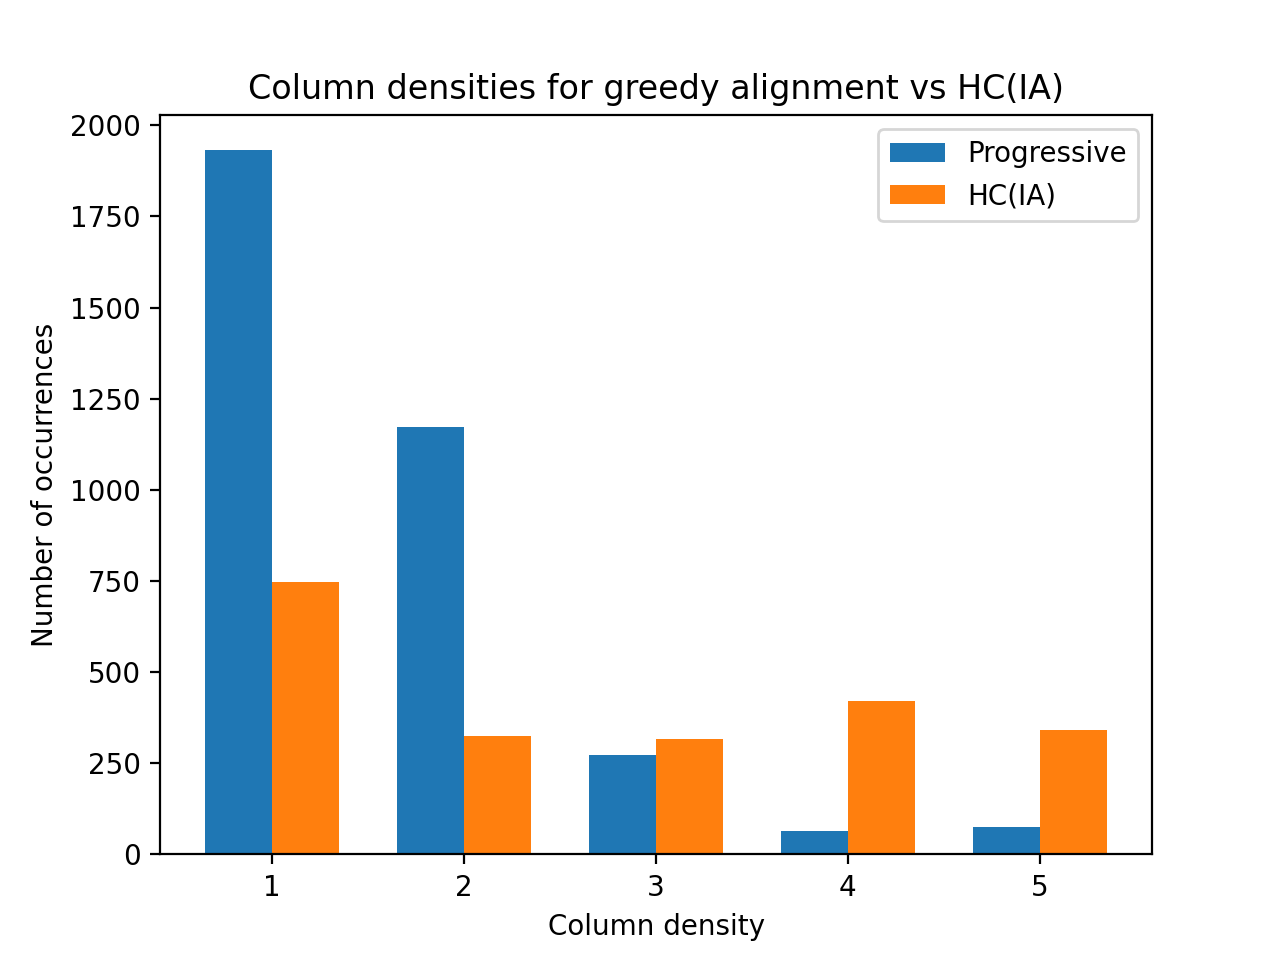
\includegraphics[width=3in]{img/prog125vhcia}
\caption{
\label{fig:colcounts}
The progressive algorithm outputs alignments that are much sparser
and longer than the best-performing method that optimizes the Steiner distance,
hill climbing (IA).
This is shown by a large number of columns from progressive alignments
containing only a single non-gap element,
and few columns containing more than 3 non-gap elements.
These column density counts were obtained across all multiple alignments from the
initial 50 clusters.
}
\end{figure}

We compare the method with the best SP score, the progressive alignment,
with the best method in terms of Steiner distance, the hill climbing algorithm
initialized with the output of iterative averaging (IA).
The alignments obtained from the progressive alignments are longer and contain more gaps
than the hill climbing (IA) alignments.
This is shown in Figure~\ref{fig:colcounts},
where the total number of columns is much larger for progressive than HC(IA),
and the column densities are lower for progressive as well.
We find that the hill climbing algorithm aligns sentences
that are not semantically similar,
therefore we focus on analyzing the progressive alignments for evidence of
storylines.

\begin{comment}
\subsection{Analysis?}
Question: Is there a bias in the alignment scores due to SBERT?
Observation: Many of the aligned sentences are short in length when sorting by star distance.
Subquestion: Are longer sentences farther from other sentences under SBERT?
\end{comment}

We observe that stories with very short sentences result in better qualitatively better alignments.
This is corroborated by Figure~\ref{fig:len-v-dist}, where the average distance
from short sentences to their nearest neighbours is smaller than that of longer sentences.
The shorter sentences may be better semantic matches,
or there may be out-of-domain issues with the sentence representations from SBERT.
The datasets SBERT was trained on were obtained from image captioning and other sources
that may not transfer well to the particular setting of the subreddit where
\textsc{WritingPrompts} was collected from;
additionally, the average sentence lengths for the datasets SBERT were trained on were 
14.1 and 22.3 \citep{bowman2015snli,williams2017mnli}
whereas the average length of sentences in the \textsc{WritingPrompts}
dataset is 28.4 \citep{fan2018writingprompts}.
We posit that SBERT has less exposure to longer, more complex (or ill-formed) sentences
such as those found in \textsc{WritingPrompts}.
The result of this bias is that shorter sentences are more likely to be matched,
and stories that contain many short sentences (especially those with many trivial nearest neighbours)
may be favored.
\begin{figure}[h]
\centering
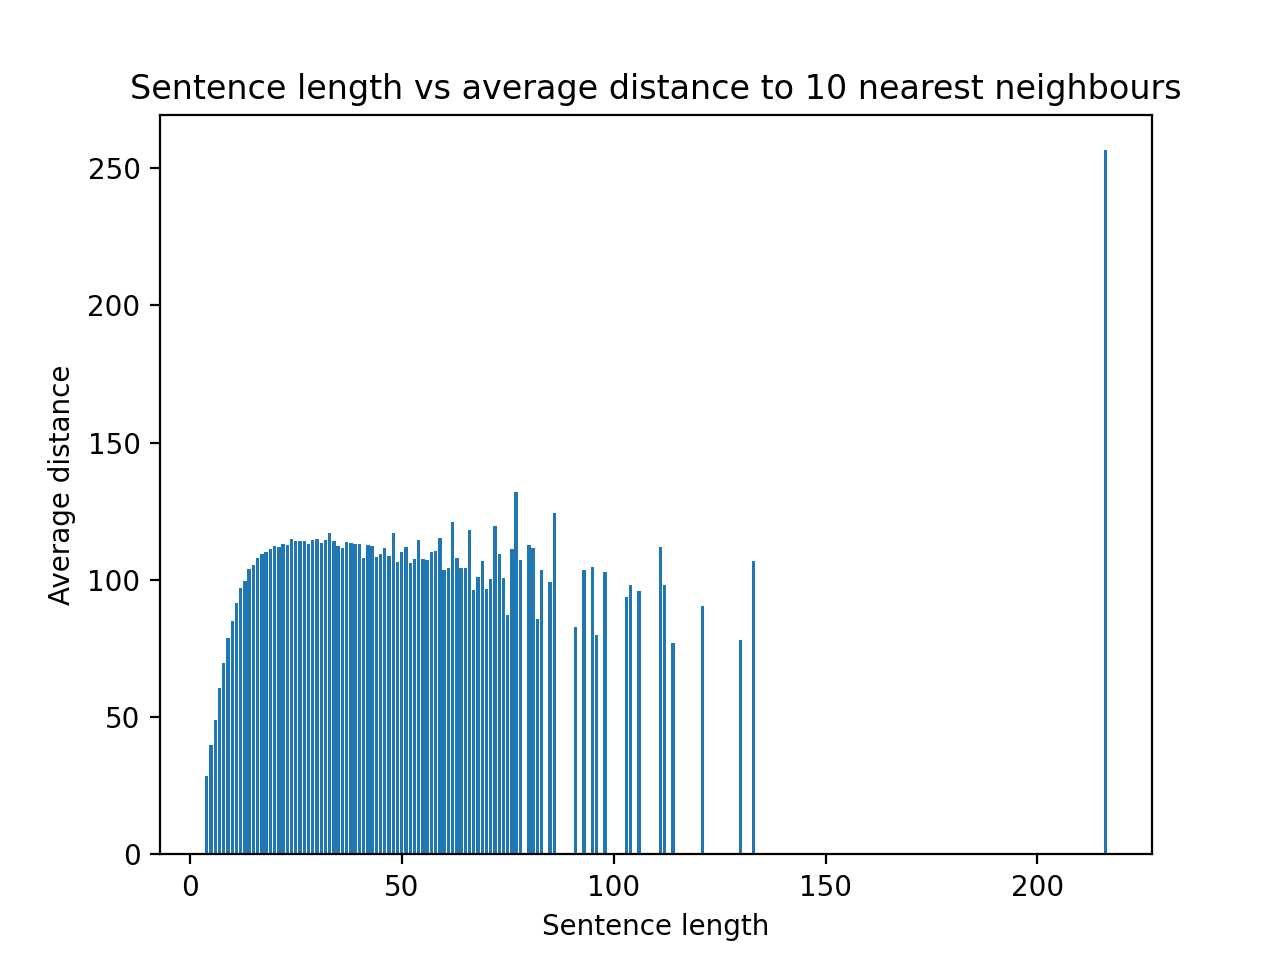
\includegraphics[width=3in]{img/senlen-v-nn-dist.png}
\caption{
\label{fig:len-v-dist}
Longer sentences tend to be farther from their nearest neighbours.
$2^{16}$ random sentences were sampled from \textsc{WritingPrompts},
and the plot shows their length versus the average distance to their 10 nearest neighbours.
Distances were averaged across all sentences of the same length.
}
\end{figure}
\begin{comment}
Subquestion: How many false negatives are we seeing because of low gap penalty?
Subquestion: Are there other measures of diversity? (maybe using kmeans clusters)
Aside: The alignments for literary criticism are quite good. This is because the sentences are statements.
    Likely closer to domain SBERT was trained on.

Question: What patterns surface through the alignments?
Subquestion: Are the sentences syntactically similar?
No. See row 12 of 3167.
Subquestion: Can we interpret aligned segments as serving a similar function in the story?
\end{comment}

However, despite the sentence-level complexity of \textsc{WritingPrompts},
the stories themselves tend to have very simple structure.
Due to their status as short stories, the traditional exposition, rising action,
falling action, and conclusion segmentations do not fit very well.
The short stories condense the structure and combine or completely leave out parts.
Additionally, as we truncate stories at 25 sentences, we may miss the conclusion
as well as the falling action.

With the SBERT and data limitations in mind, we examine a particular set of 5 stories 
with nontrivial alignments as a case study.
The prompt and first few sentences of each story are given in Figure~\ref{fig:story-starts}.
We find that the initial heuristics for finding sets of stories using the bigram BoS representations,
and subsequently the pairwise alignment distances is effective at finding similar stories.
As the stories in our case study cluster are all about outer space, we refer to them as
the space story cluster.
The multiple alignment for the cluster, in Figure~\ref{fig:msa},
although sparse, shows some evidence of storylines.
Indices 1-14 of the alignment appear to be the introduction of stories 1, 2, 3, and 5,
with story 4 taking a less conventional structure and style.
Due to their nature as short stories, much of the remainder of the stories fall under exposition:
the stories unfortunately do not obey the rule ``show don't tell''
so it is difficult to distinguish exposition from action.

We present a good sub-alignment in Figure~\ref{fig:good-alignment},
which involves indices 11 and 12 in Figure~\ref{fig:msa}.
This particular alignment occurs early in the multiple alignment,
and captures shared structure across four of the five stories
and marks the end of the introduction section mentioned previously.

We also examine a poor sub-alignment in Figure~\ref{fig:bad-alignment},
which involves indices 31-34 from the multiple alignment.
The fragment from story 4 occurs towards the end that story's introduction,
yet is aligned to sentences that occur after story 5's introduction.
We hypothesize that story 4 is dissimilar to the other four stories,
causing errors in the alignment.

The full multiple alignment for this cluster, as well as other clusters,
can be viewed by following the instructions at the following site:
\href{https://github.com/dongruoping/story-clustering/}{github.com/dongruoping/story-clustering}.

\begin{figure}[h]
\centering
\small
\begin{tabular}{|p{\textwidth}|}
\hline
\textbf{Story 1}
\\
\hline
\\
\textit{After hundreds of years of sending messages into the sky , humanity receives its first message from intelligent life . Decoded it simply says , `` Be quiet before they find you . ''}
\\
\\
'' Zebin exclaimed as he received yet one more channel of communication from the Earth .
Twenty years ago , the ambivalence over whether KIC 8462852 was in actuality an `` alien mega structure '' had finally come to an end after nearly 200 years of joint scientific endeavour by the leading lieges of the Earth .
Since then , humanity had been trying with fervor to try and communicate with the star classified as a Dyson Sphere around 1480 light years away hoping that the far advanced civilisation might be generous enough to show the earthlings a way to solve their own energy crisis .
\\
\hline
\textbf{Story 2}
\\
\hline
\\
\textit{Sunday Free Write : Leave A Story , Leave A Comment - New CSS Edition !}
\\
\\
In 2056 NASA intercepted a frequency that was not of Earth .
With its point of origin unknown they began to study it in an attempt to discover from whence it came .
As it was studied it became known as the whoa signal , mockingly after the famous `` wow !
\\
\\
\hline
\textbf{Story 3}
\\
\hline
\\
\textit{By 2345 humanity has colonized most of the solar system and have started sending probes beyond sol , when one day , a frantic interstellar message is received saying `` do not leave the sol system ''}
\\
\\
Listen well childen , for I have a Story of Old Earth to tell .
Long ago , in ages past , the Men of ages past had but one True world , and had not yet learned to truely swim across the stars .
In the nuturing embrace of Sol , humanity sowed life in the wake of the places Man gone .
\\
\\
\hline
\textbf{Story 4}
\\
\hline
\\
\textit{As the universe resonates for its final time , heat death approaching , the last energy of the universe is used to send a message .}
\\
\\
We knew something was going on , we knew something at any time would happen as time went on .
Millennia after millennia we saw the lights fade out year by year pondering if new ones will be born to re-convey balance in the universe , but no the night sky kept getting darker star by star .
We did n't care at first but the scientists all around our universe that we spread around knew something was wrong but were too busy with inorganically creating life on a possibly inhabitable planet around Zylon-B .
\\
\\
\hline
\textbf{Story 5}
\\
\hline
\\
\textit{Astronauts discover an abandoned space station orbiting a small moon . It is the far future .}
\\
\\
“ Alright , we ’ re here , ” Captain Schiff said as the blocky craft approached the small disc-like object orbiting around Io , one of the five Galilean moons of Jupiter .
An astronomer working for Global Colony Services , GSC , a young but highly profitable organization with fledgling colonies on the Moon , Mars , and in the asteroid belt , had spotted an irregular object in lunar-synchronous orbit that wasn ’ t there last year .
The GSC , or rather the league of nations sponsoring it , was concerned about a potential threat to the admittedly massive investments it had made in the asteroid belt , so it had sent the great ship MecaBubo 1 out to investigate .
\\
\hline
\end{tabular}
\caption{
\label{fig:story-starts}
The first few sentences from each of the 5 stories in our space story cluster analysis.
The prompt is for each story is given in italics.
All stories have a space-related theme.
The first two sentences of story 5 have been filtered out, as they repeated the prompt.
}
\end{figure}

\begin{figure}[h]
\centering
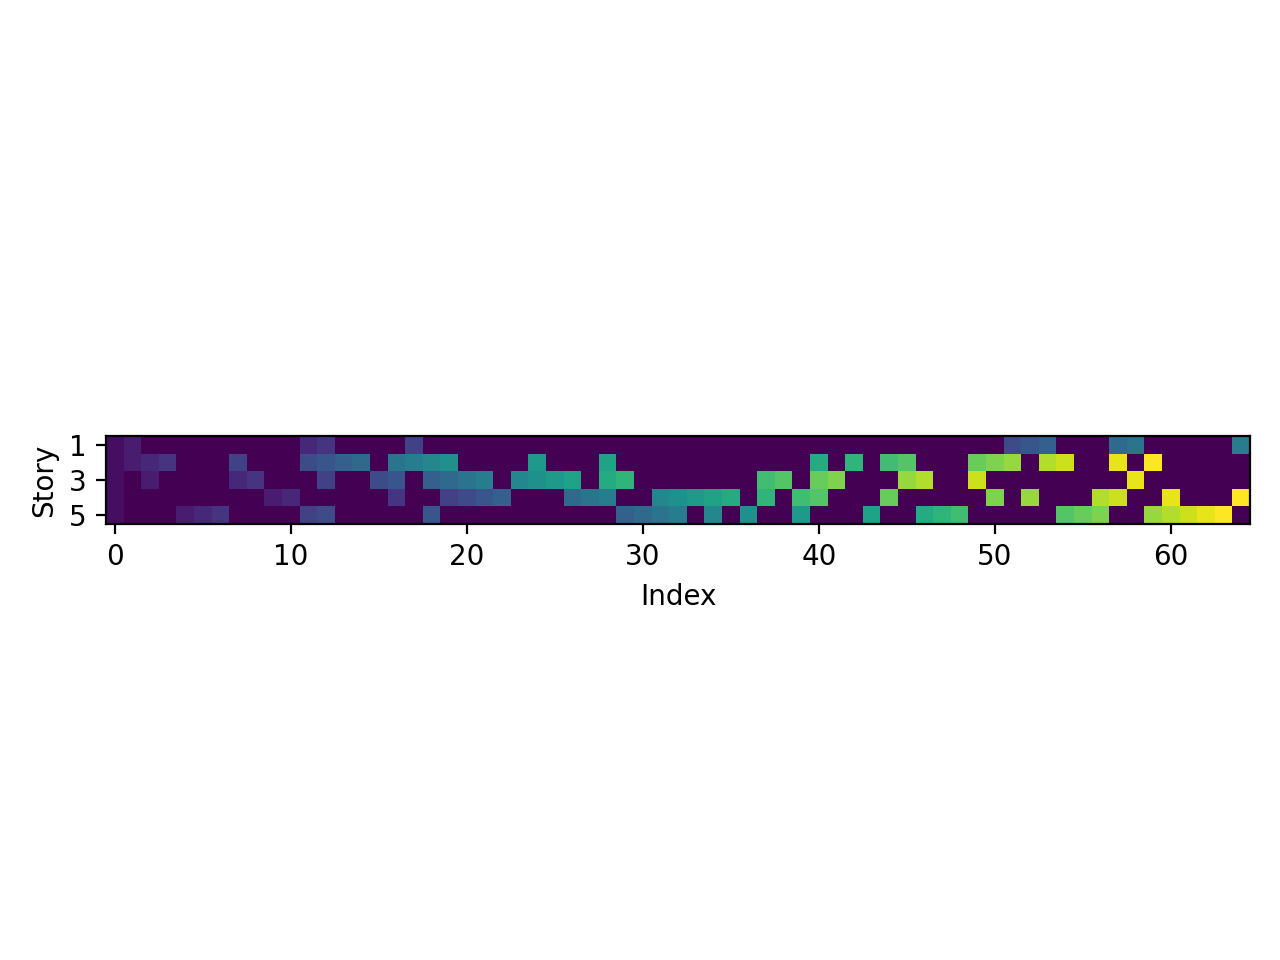
\includegraphics[width=5in,trim=0em 12em 0em 12em,clip]{img/msa3167.png}
\caption{
\label{fig:msa}
The multiple story alignment of the space story cluster, obtained via progressive alignment.
We refer to the story in the top-most row as story 1, down through the bottom-most row
as story 5.
Each colored square corresponds to a sentence from the corresponding story,
while a dark square corresponds to a gap.
Sentences within a row proceed in order of their appearance in the story;
only gaps are inserted within each row.
An identical dummy beginning-of-story sentence token was inserted at the start of each story,
yielding the full column of matches at index 0.
}
\end{figure}


\begin{figure}[h]
\centering
\small
\begin{tabular}{|p{0.25\textwidth}|p{0.25\textwidth}|p{0.25\textwidth}|p{0.25\textwidth}|}
\hline
\textbf{Story 1} & \textbf{Story 2} & \textbf{Story 3} & \textbf{Story 5}
\\
\hline
 Twenty years ago , the ambivalence over whether KIC 8462852 was in actuality an `` alien mega structure '' had finally come to an end after nearly 200 years of joint scientific endeavour by the leading lieges of the Earth .
& NASA discovered the signal was encrypted like nothing they had ever dreamed of ; the discovery of the encryption itself set technology hundreds of years ahead of where it once was .
&& An astronomer working for Global Colony Services , GSC , a young but highly profitable organization with fledgling colonies on the Moon , Mars , and in the asteroid belt , had spotted an irregular object in lunar-synchronous orbit that wasn ’ t there last year .
\\
\hline
Since then , humanity had been trying with fervor to try and communicate with the star classified as a Dyson Sphere around 1480 light years away hoping that the far advanced civilisation might be generous enough to show the earthlings a way to solve their own energy crisis .
& It sparked the golden age of exploration in our solar system ; Ceres , Vesta , Hektor , Thisbe , Diotina , Fortuna were among many asteroids in the asteroid belt that were to be mined and inhabited ; the once failed colonization of Mars was reattempted and achieved , Europa of Jupiter , Titan of Saturn and Triton of Neptune all were to be colonized and inhabited ; Man had even reached as far as the Oort Cloud in the outer reaches of our solar system as early as 2096 .
& From the Illiuminious research Stations of Mercury , to the Ruins of Old Chicago , Humanity had taken to the space around Sol with great bravado .
& The GSC , or rather the league of nations sponsoring it , was concerned about a potential threat to the admittedly massive investments it had made in the asteroid belt , so it had sent the great ship MecaBubo 1 out to investigate .
\\
\hline
\end{tabular}
\caption{
\label{fig:good-alignment}
An example of a good alignment between 4 story segments from the multiple alignment.
The first sentences from stories 1, 2, and 5 detail an event which sparked the following sentences.
The next sentences from all four stories mention a form of exploration, investigation, or expansion.
}
\end{figure}


\begin{figure}[h]
\centering
\small
\begin{tabular}{|p{0.5\textwidth}|p{0.5\textwidth}|}
\hline
\textbf{Story 4} & \textbf{Story 5}
\\
\hline
We tried making stars but they all died out faster then the stars above but it seemed somehow to make our time last just a little bit longer .
& Not even great technicians at that, since the ship could handle damn near everything itself .
\\
\hline
We had time to formulate whats going on and a joint meeting of scientists from all around the corners of the universe .
& We were there as human eyes and ears , witnesses to send back any special details , in case they were necessary , and mechanics to fix the ship in case one of those “ one in a million ” scenarios cropped up ( which seemed to be happening more and more often since children of Adam and Eve began to colonize their small corner of the cosmos .
\\
\hline
Some full robotic now , half robotic and humanoid , one was full humanoid from Earth 1B and some that looked so foreign from living on a planet with no sunlight for 3 years at a time with the vegetation growing above 40 feet in the air .
& \\
\hline
Enough about the scientists though .
& Schiff was our leader , and a good enough man , if a bit formal .
\\
\hline
\end{tabular}
\caption{
\label{fig:bad-alignment}
An example of a poor alignment between two story segments from the multiple alignment.
The sentences are weak semantic matches, although both segments
serve as exposition in their respective stories.
}
\end{figure}

\section{Discussion}
We present a comparison of objectives and algorithms for performing multiple alignment,
with the goal of inducing storylines.
We find that progressive alignment results in the best alignment qualitatively.
Analysis of the output of the progressive revealed some structure in stories,
but the results were also obscured with noise from three possible sources:
1) suboptimal choices of story sets, 2) suboptimal alignments from the algorithm, 
and 3) behaviour of the sentence representations obtained from SBERT on out-of-domain data.
For our next step, we will improve the accuracy and scalability of our alignment algorithm
in order to apply it to even larger subsets of stories, addressing problems 1 and 2.
We hypothesize that by increasing the number of stories aligned, we will be able to 
improve the quality of the alignments by decreasing the probability of outlier stories with no similar stories in the same set.

\newpage
\bibliographystyle{plainnat}
\bibliography{bib}

\end{document}
